\documentclass[11pt,a4paper]{ltjsarticle}
% Compile with LuaLaTeX

% =========================
% Packages
% =========================
\usepackage{luatexja}
\usepackage{graphicx}
\usepackage{hyperref}
\usepackage{amsmath,amssymb,mathtools}
\usepackage{xcolor}
\usepackage{float}
\usepackage{subcaption}
\usepackage{booktabs}
\usepackage{enumitem}
\usepackage{geometry}

\geometry{margin=22mm}
\setcounter{tocdepth}{3}
\setlength{\parskip}{0.6mm}

% =========================
% User information
% =========================
\title{Weekly Report: Ultra-High-Pressure ODMR --- \\ How much of the predicted multiplicity ladder can we actually measure?}
\author{Risei Abe}
\date{Week: 2026/08/24 -- 2026/08/30}

% =========================
% Custom commands
% =========================
\newcommand{\sectionblock}[1]{%
  \vspace{2mm}
  {\large\textbf{#1}}
  \vspace{1mm}

}

\newcommand{\todo}[1]{\textcolor{red}{#1}}

\begin{document}

\maketitle

% =========================================================
% 1. Question / Purpose
% =========================================================
\sectionblock{Question}

\begin{quote}
Theorem M says the optimal excitation wavelength above the splitting power $I_c$ is not a point but a level set of the absorption kernel, whose size $N$ is a step function of power ($N = 2,4,6,4,3,5,3$ at 120\,GPa); since a level set is degenerate by construction, what an experiment sees is not $N$ but the $\eta$ \emph{bump between} its members --- so how many rungs survive finite wavelength resolution and finite photometric precision, and what power grid do the survivors demand?
\end{quote}

% =========================================================
% 2. Hypothesis
% =========================================================
\sectionblock{Hypothesis}

If two members closer than the addressable wavelength resolution ($0.5$\,nm; the pair straddling the zero-phonon line is only $0.1$\,nm apart) merge into one observed optimum, and if a rung counts as read only when every bump separating its members clears $3\sigma_\eta$, then the observable ladder should be strictly shorter than the mathematical one, and the grid should be set by the narrowest \emph{readable} rung rather than by the narrowest rung --- so tightening $\sigma_\eta$ should buy rungs discontinuously and at a steeply rising cost in points.

% =========================================================
% 3. Evidence / Interpretation
% =========================================================
\sectionblock{Evidence / Interpretation}

\begin{figure}[H]
  \centering
  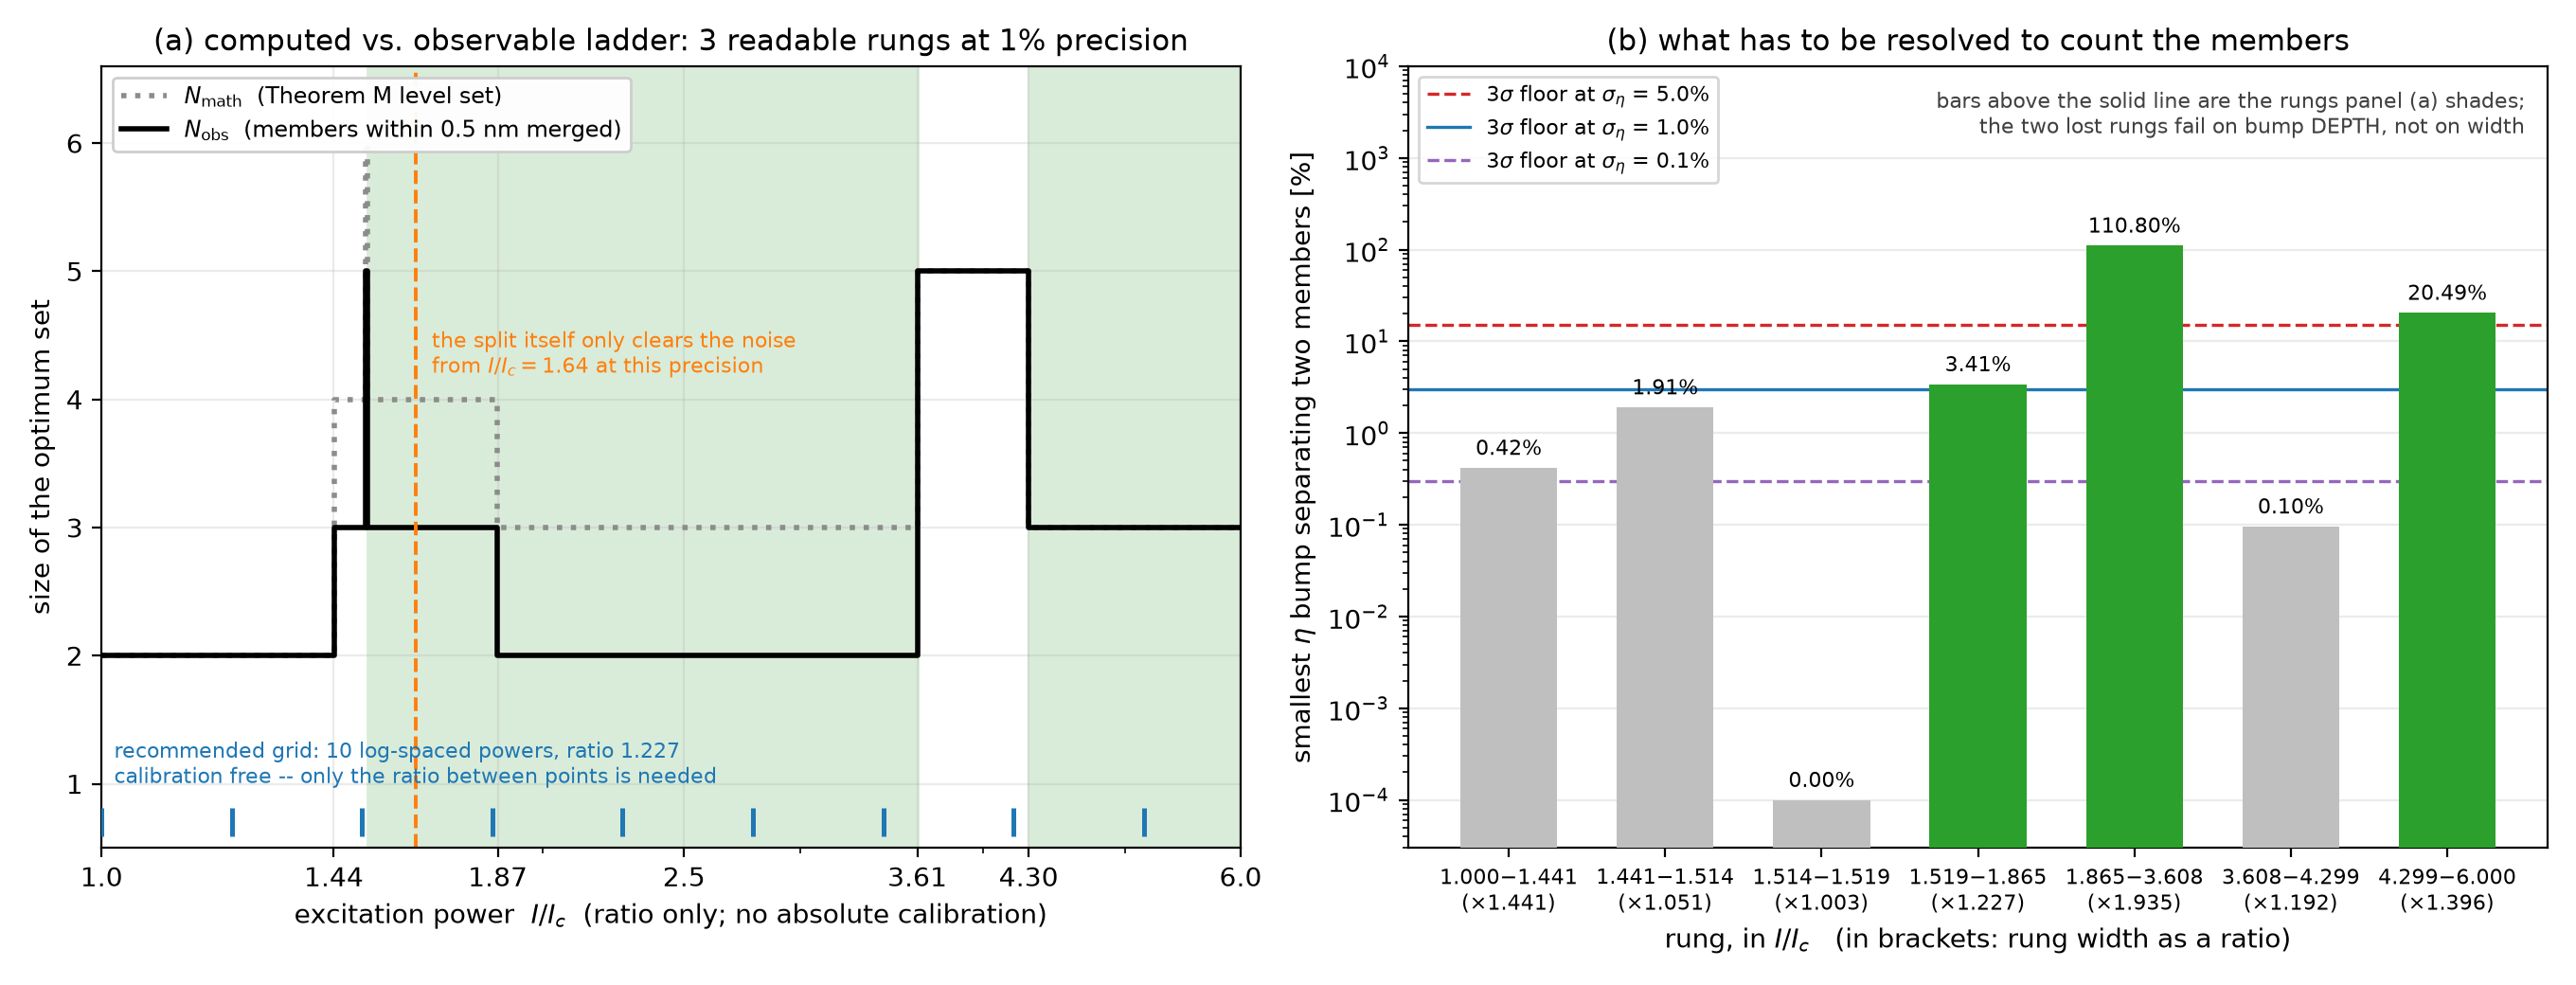
\includegraphics[width=0.98\linewidth]{image/ladder_detection.png}
  \vspace{-1mm}
  \caption{(a) The ladder as Theorem M computes it ($N_{\rm math}$) and as an experiment sees it ($N_{\rm obs}$, members within $0.5$\,nm merged); shading marks the rungs readable at $\sigma_\eta = 1\%$, ticks the recommended ten-point grid. (b) The smallest $\eta$ bump on each rung against the $3\sigma$ detection floor; bar labels give the bump, brackets the rung width.}
  \label{fig:ladder}
\end{figure}
\vspace{-3mm}

\begin{itemize}[leftmargin=8mm]
  \item Resolution alone shortens the ladder to $N_{\rm obs} = 2,3,5,3,2,5,3$, but the binding filter is bump depth, which spans four orders of magnitude ($0.00\%$ to $110.80\%$). At $\sigma_\eta = 1\%$ exactly three rungs are readable --- $I/I_c = 1.519$--$1.865$, $1.865$--$3.608$ and $4.299$--$6.000$ --- and the $\times 1.192$-wide five-member rung at $3.608$--$4.299$ is lost to depth ($0.10\%$), not to width, which the freeze had not anticipated.
  \item The narrowest readable rung ($\times 1.227$) fixes the grid: \textbf{ten log-spaced powers from $I/I_c = 1$ to $6$, ratio $1.227$}, with $0\%$ probability of stepping over any of the three readable rungs. Because the transition powers are the calibration-free ratios $I_k/I_c = A_{\max}/A_k$, the grid needs only the \emph{ratio} between points, not absolute laser power --- what it does need is span, $I_{\max}/I_c \ge 4.3$.
  \item Precision buys rungs in jumps and not cheaply: $5\%$ and $2\%$ both give two rungs in seven points, $1\%$ gives three in ten, and $0.5\%$ gives four but drops the binding width to $\times 1.051$ and so demands \textbf{38} points.
  \item \textbf{The headline claim is the hardest thing to see.} The split opens continuously from zero at $I_c$ ($0.005\%$ at $I/I_c = 1.02$, $1.7\%$ at $1.44$), so at $1\%$ it only clears $3\sigma$ from $I/I_c \approx 1.64$, and ``we saw the optimum divide'' needs sub-$0.1\%$ photometry. The robust observables are the \emph{later} transitions at $1.865$ and $4.299$, where the zero-phonon line enters and the bumps exceed $100\%$ and $20\%$. The experiment should therefore be aimed at ``the multiplicity changed at the predicted calibration-free power ratios,'' not at the split itself.
\end{itemize}

% =========================================================
% 4.  Gap / Failure
% =========================================================
\sectionblock{Gap / Failure}

\begin{itemize}[leftmargin=8mm]
  \item The bump depths --- unlike the level-set structure, which is kernel independent --- are computed from the Ho Fig.\,1(e) kernel reconstruction, so every number in Fig.\,\ref{fig:ladder}(b) is an L2 (kernel-conditional) illustration; the $0.5$\,nm resolution and the $3\sigma$ criterion are assumed rather than measured on our bench.
  \item The grid is calibration free but the \emph{span} is not: reaching the last readable rung needs $I_{\max}/I_c \ge 4.3$, and $I_c$ (about $7\%$ of saturation in the model) has never been located experimentally, so we cannot yet say whether our source has the headroom.
  \item Assumption (M) is still untested, and its live failure candidate --- charge-state partitioning, with $405$\,nm favouring NV$^0$ at low pressure (Bhattacharyya, p.\,65) --- would act precisely on the level-set members this experiment counts.
  \item Scope is unchanged and narrow: [111] culet, [111] NV group, sample chamber; and anvil transmission clears its threshold by only $1.9\sigma$ for type Ia, with the DAC-side type Ib case unmeasured.
\end{itemize}

% =========================================================
% 5. Next Step
% =========================================================
\sectionblock{Next Step}

Run the ten-point calibration-free power sweep at 120\,GPa with $1\%$ photometry on $\eta$, aiming at the transitions at $I/I_c = 1.865$ and $4.299$ rather than at the split; and, at each member of the observed optimum set, record the NV$^0$/NV$^-$ ratio in the same sweep, since that is the one measurement that tests assumption (M) at no extra cost in beam time. Locating $I_c$ (the onset of any splitting at all) is the first point of that sweep and settles whether the $\ge 4.3$ span is reachable.

% =========================================================
% 9. References
% =========================================================
\sectionblock{References}

\begin{enumerate}[leftmargin=8mm]
  \item K.\,O.\ Ho, C.\ Dailledouze, V.\ \v{Z}alandauskas, \emph{et al.}, ``Optical Stability and Photophysics of NV Centers in Diamond up to 120 GPa,'' arXiv:2606.02399 (2026).
  \item A.\ Dr\'eau \emph{et al.}, ``Avoiding power broadening in optically detected magnetic resonance of single NV defects,'' Phys.\ Rev.\ B \textbf{84}, 195204 (2011).
  \item P.\ Bhattacharyya, \emph{Principle and Applications of Quantum Metrology in Diamond Anvil Cells using the Nitrogen Vacancy Color Center}, Ph.D.\ thesis, UC Berkeley (Fall 2022), Ch.\ 6 and p.\,65.
  \item Repository: \texttt{code/ladder\_detection.py}, \texttt{code/theory\_a2\_multiplicity.py}, \texttt{code/fig10\_ladder\_detection.py} (this analysis); \texttt{theory\_freeze\_v3\_ho\_integrated.md} (A2, N1--N4), \texttt{STATUS.md} \S6.
\end{enumerate}

\end{document}
